\documentclass[10pt,aspectratio=169]{beamer}

\usetheme{Madrid}
\usecolortheme{seahorse}
\setbeamertemplate{navigation symbols}{}
\setbeamertemplate{footline}[frame number]
\setbeamertemplate{itemize items}[circle]
\setbeamercolor{title}{fg=white,bg=black!80!green}
\setbeamercolor{frametitle}{fg=white,bg=black!75!green}

\usepackage{fontspec}
\setmainfont{Noto Sans}
\usepackage{amsmath,amssymb}
\usepackage{graphicx}
\usepackage{booktabs}
\usepackage{tikz}
\usetikzlibrary{arrows.meta,positioning,shapes.geometric,fit,calc,backgrounds}

\definecolor{cudaG}{RGB}{118,185,0}
\definecolor{sadRed}{RGB}{200,60,50}
\definecolor{gsBlue}{RGB}{40,110,190}
\definecolor{pyYel}{RGB}{240,170,30}
\definecolor{bgGray}{RGB}{242,242,242}

\newcommand{\keybox}[2][cudaG]{%
  \begin{tikzpicture}
    \node[draw=#1,line width=1pt,rounded corners,fill=#1!10,inner sep=6pt,text width=0.92\textwidth,font=\small] {#2};
  \end{tikzpicture}}


\title[Render 3D for BTS Stations]{Rendering a BTS Station in 3D\[2pt]
\large From the CUDA rasterizer to SADGS: a digital twin for telecom sites}
\author{30-minute talk}
\date{\today}

\begin{document}

\begin{frame}
  \titlepage
\end{frame}

\begin{frame}{Outline}
  \tableofcontents
\end{frame}

\section{Problem and results}
\input{sections/s01}

\section{CUDA foundations}
\begin{frame}{GPU execution model: grid, block, warp, thread}
  \centering
  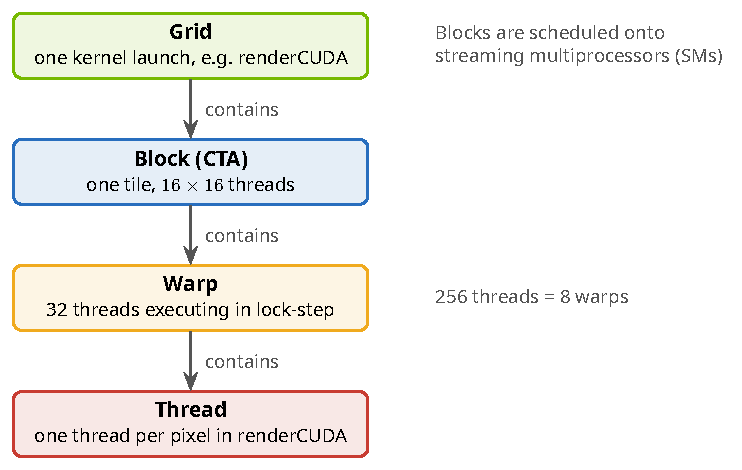
\includegraphics[width=0.95\textwidth,height=0.62\textheight,keepaspectratio]{figs/s02_1.pdf}\\[2pt]
  {\small
  \begin{itemize}
    \item A kernel launch creates a \textbf{grid} of \textbf{blocks}; each block runs on one SM.
    \item In the rasterizer, one block handles one $16\times16$ tile.
    \item A block is split into 32-thread \textbf{warps}; 256 threads give 8 warps.
  \end{itemize}}
\end{frame}

\begin{frame}{Mapping pixels to threads: one tile per block}
  \centering
  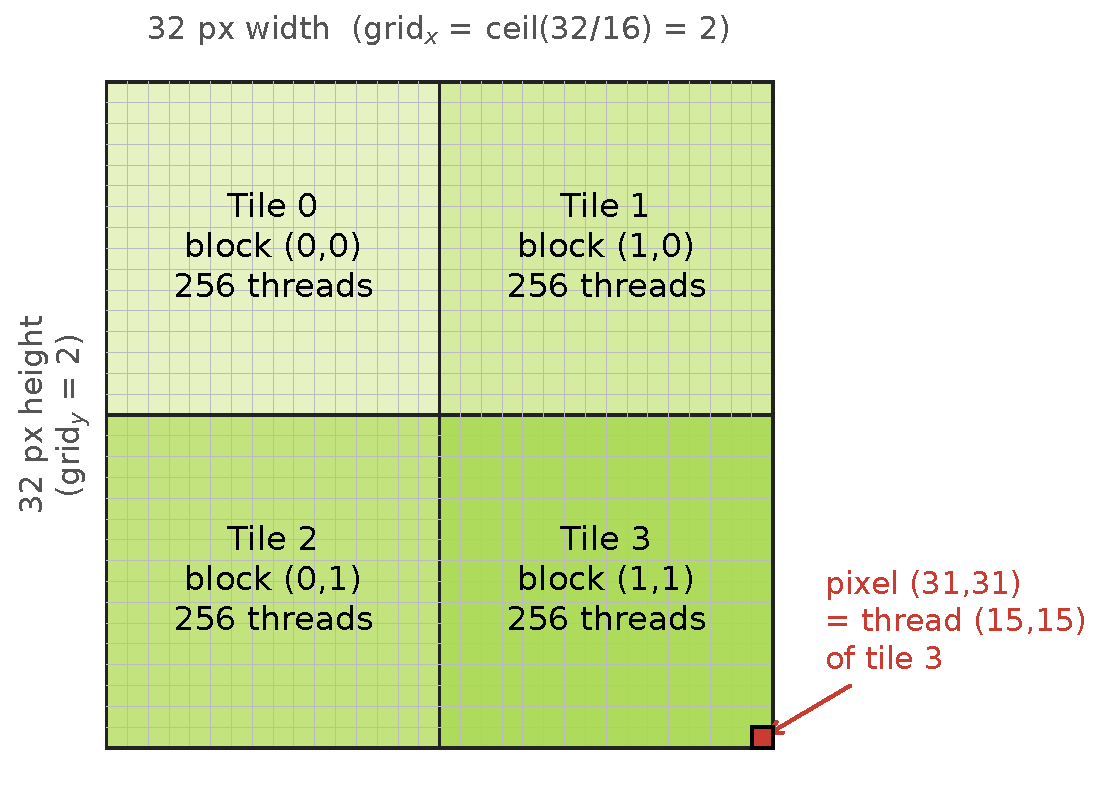
\includegraphics[width=0.95\textwidth,height=0.62\textheight,keepaspectratio]{figs/s02_2.pdf}\\[2pt]
  {\small
  \begin{itemize}
    \item \texttt{BLOCK\_X = BLOCK\_Y = 16}, so one block = 256 threads = one tile.
    \item Grid size: $\mathrm{grid}_x=\lceil W/16\rceil$, $\mathrm{grid}_y=\lceil H/16\rceil$.
    \item Example: $32\times32$ image gives a $2\times2$ grid, i.e.\ $n=4$ tiles. Each thread shades one pixel.
  \end{itemize}}
\end{frame}

\begin{frame}{CUDA memory hierarchy}
  \centering
  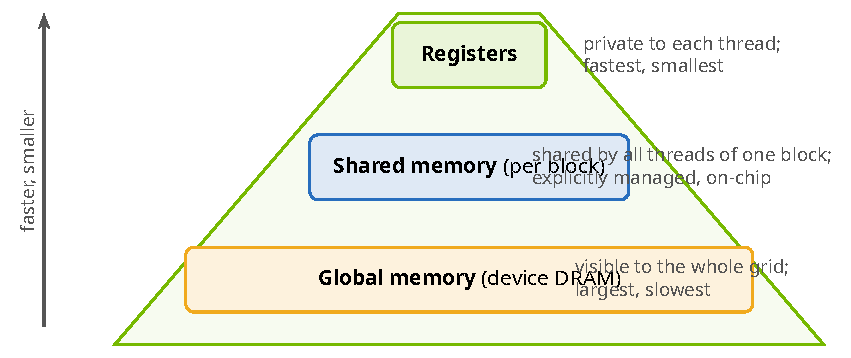
\includegraphics[width=0.95\textwidth,height=0.62\textheight,keepaspectratio]{figs/s02_3.pdf}\\[2pt]
  {\small
  \begin{itemize}
    \item \textbf{Registers}: private per thread, fastest.
    \item \textbf{Shared memory}: per block, managed explicitly by the kernel.
    \item \textbf{Global memory}: whole device, holds the Gaussian parameters and the image buffers.
    \item Design goal: keep the hot per-Gaussian data in shared memory (qualitative, no bandwidth figures here).
  \end{itemize}}
\end{frame}

\begin{frame}{Why the rasterizer batches Gaussians into shared memory}
  \centering
  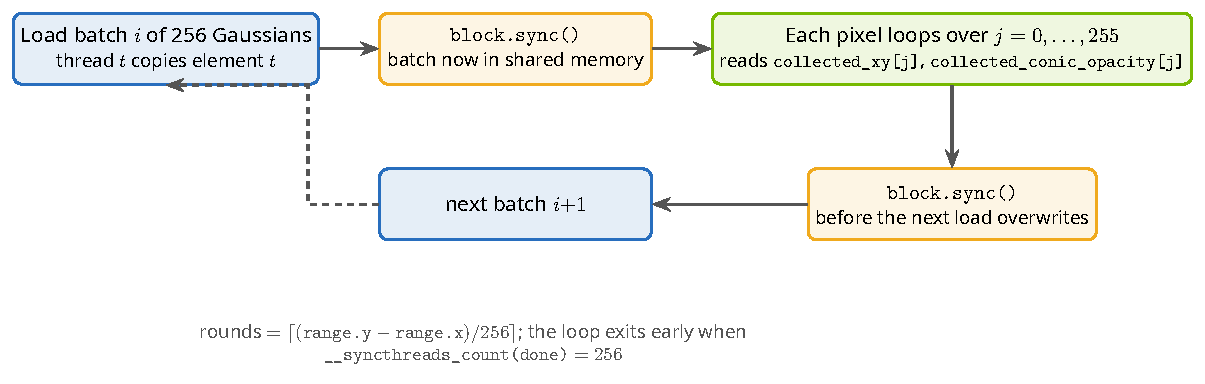
\includegraphics[width=0.95\textwidth,height=0.62\textheight,keepaspectratio]{figs/s02_4.pdf}\\[2pt]
  {\small
  \begin{itemize}
    \item Each batch holds \texttt{BLOCK\_SIZE = 256} Gaussians: \texttt{collected\_id}, \texttt{collected\_xy}, \texttt{collected\_conic\_opacity}.
    \item All 256 pixels of the tile read the same batch, in the same depth order.
    \item \texttt{block.sync()} before and after loading keeps the threads in step.
  \end{itemize}}
\end{frame}

\begin{frame}{Spherical harmonics: 16 coefficients per channel}
  \centering
  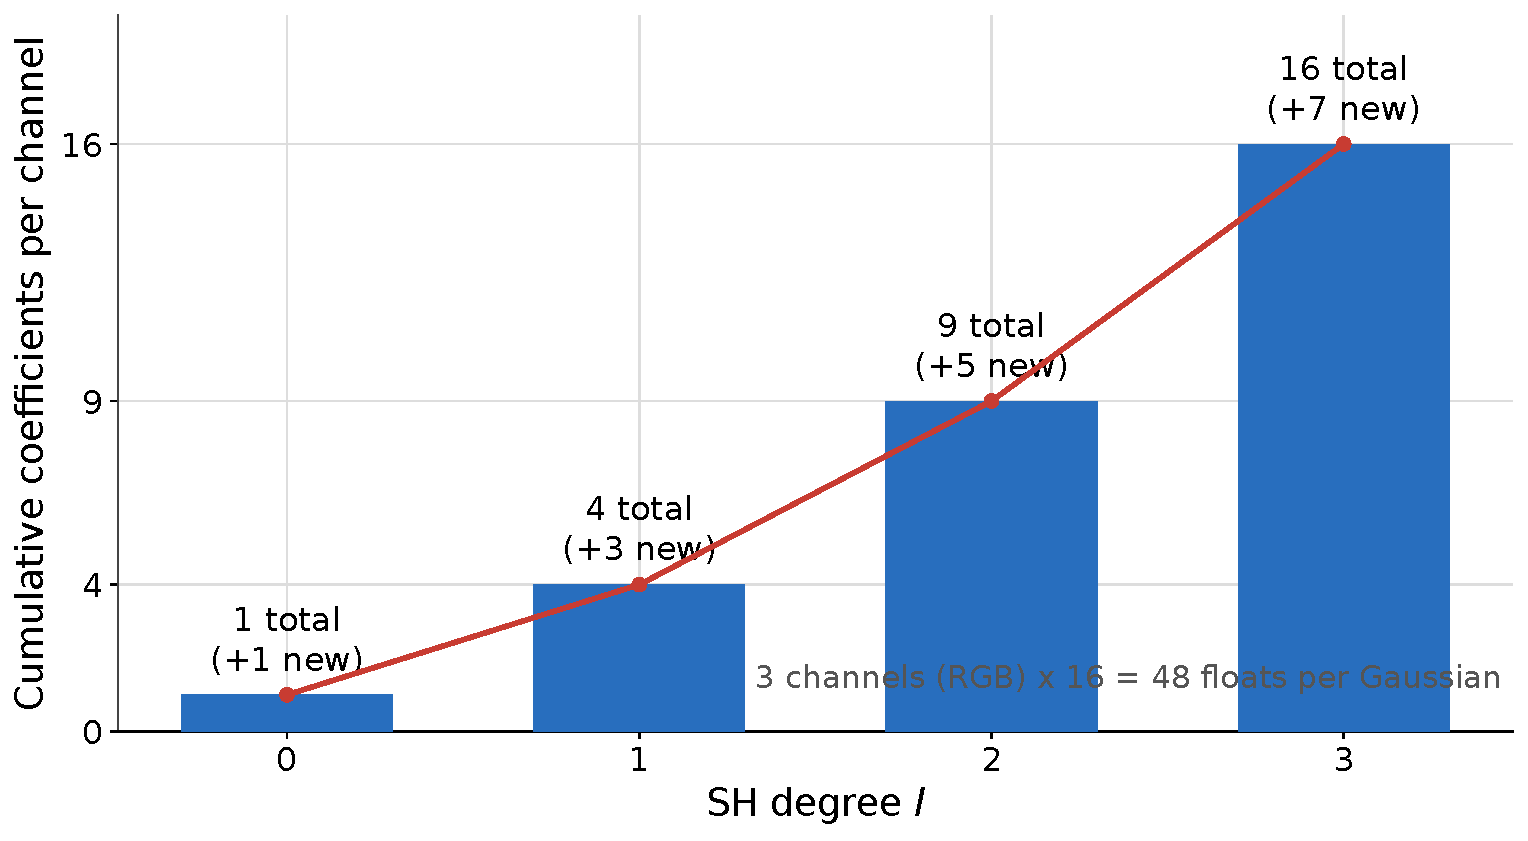
\includegraphics[width=0.95\textwidth,height=0.62\textheight,keepaspectratio]{figs/s02_5.pdf}\\[2pt]
  {\small
  \begin{itemize}
    \item Degree $l$ adds $2l+1$ basis functions: $l=0,1,2,3$ gives $1,3,5,7$.
    \item Cumulative total $1, 4, 9, 16$ per colour channel ($(\deg+1)^2$).
    \item Higher degrees add view-dependent detail; the 3DGS default uses up to $l=3$.
  \end{itemize}}
\end{frame}

\begin{frame}{\texttt{computeColorFromSH} in four steps}
  \centering
  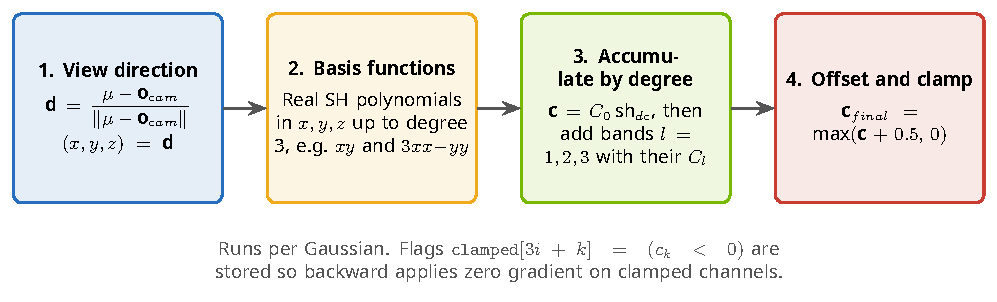
\includegraphics[width=0.95\textwidth,height=0.62\textheight,keepaspectratio]{figs/s02_6.pdf}\\[2pt]
  {\small
  \begin{itemize}
    \item Step 4 is $\mathbf c_{final}=\max(\mathbf c+0.5,\,0)$: the $+0.5$ offset and clamp to non-negative values.
    \item Coefficients: $C_0=0.28209\ldots$, $C_1=0.48860\ldots$, followed by the degree-2 and degree-3 constants.
  \end{itemize}}
\end{frame}


\section{Forward pass: from Gaussians to pixels}
\input{sections/s03}
\input{sections/s04}
\input{sections/s05}
\input{sections/s06}

\section{Backward pass: gradients back to Gaussians}
\input{sections/s07}
\input{sections/s08}
\input{sections/s09}

\section{SADGS and applications}
\input{sections/s10}

\begin{frame}
  \centering
  {\Large Thank you --- Questions?}\[6pt]
  {\footnotesize Sources: \texttt{MATH/submodules/diff-gaussian-rasterization\_structgs/}, \texttt{DOCS/BOOK/}, \texttt{bts\_digital\_twin.ipynb}}
\end{frame}

\end{document}
